\section{Measuring Structural Complexity }\label{sec:meaComplex}

The goal of the section is to describe our solution to the challenging
problem of estimating the entropy of an arbitrary, real-valued time
series.  This approach draws upon methods and results from a variety
of fields including time-series analysis, dynamical systems, and
stochastic processes.

For the purposes of this paper, we view the Shannon entropy---in
particular its growth rate with respect to word length (the
\emph{Shannon entropy rate})---as a measure of complexity and
unpredictability in a time series.  Time-series consisting of IID 
random variables, such as white noise, have maximal entropy rates, 
whereas highly structured time-series, for example periodic, have very
low or zero entropy rate. A time series with a high entropy rate is 
almost completely unpredictable; conversely one with low entropy rate
is often quite predictable. This can be made more rigorous: Pesin's
relation \cite{pesin77} states that in chaotic dynamical systems, the
Kolmogorov-Sinai (KS) entropy is equal to the sum of the positive
Lyapunov exponents, $\lambda_i$.  The Lyapunov exponents directly
quantify the rate at which nearby states of the system diverge with
time: $\left| \Delta x(t) \right| \approx e^{\lambda t} \left| \Delta
x(0) \right|$.  The faster the divergence, the larger the entropy, and
the more difficult prediction becomes.  The KS entropy is defined as
the supremum of the Shannon entropy rates of all
partitions~\cite{petersen1989}. The partition that achieves this
supremum is the \emph{generating partition} discussed in
Section~\ref{sec:related}.

From a different point of view, we can consider the information (as
measured by the Shannon entropy) contained in a single observable, say
the \emph{present}, of the system. This information can be partitioned
into two components: the information shared with past
observations---e.g., the mutual information between the past and
present---and the information in the present that is not contained in
the past (aka ``the conditional entropy of the present given the
past'').  The first part is known as the \emph{redundancy}, as it is
information in the present which is also in the past.  The second part
is the aforementioned \emph{Shannon entropy rate}.  We conjecture that 
the more redundancy in a signal, the more predictable it is.  
Redundancy is critical to prediction, in general.  And the specific 
\emph{form} of the redundancy dictates whether a particular prediction 
method will work well or poorly on the corresponding signal.  A linear 
method cannot detect or make use of nonlinear redundancy, for 
instance.  This issue is central to the claims in this paper and the 
discussion in the following section.

Utilizing Shannon entropy rate as a measure of temporal complexity is
not a new idea \cite{Shannon1951, mantegna1994linguistic}, but
previous approaches required categorical data: $x_i \in \mathcal{S}$
for some finite or countably infinite \emph{alphabet} $\mathcal{S}$.
Data taken from real-world systems is, however,
effectively\footnote{Measurements from finite-precision sensors are
  discrete, but data from modern high-resolution sensors are, for the
  purposes of entropy calculations, effectively continuous.}
real-valued.  To analyze real-valued data using a method that requires
categorical values, one must discretize the data---typically by
binning.  Unfortunately, this is rarely a good solution, as the
binning of the values introduces spurious dynamics~\cite{bollt2001}.
The field of symbolic dynamics offers discretization methods that do
not disturb the intrinsic behavior.  These methods are, however,
fragile in the face of noise; worse yet, they require knowledge of the
underlying system.  This is not useful in our context, where we want
to measure the entropy to quantify predictability.

Bandt and Pompe introduced the \emph{permutation entropy} (PE) as a
``natural complexity measure for time series''
\cite{bandt2002per}. The permutation entropy employs a method of
discretizing real-valued time series that follows the intrinsic
behavior of the system under examination, and has many advantages 
including being robust to observational noise and its application does 
not require any knowledge of the underlying mechanisms.  Rather than 
looking at the statistics of sequences of values, as is done when 
computing the Shannon entropy, permutation entropy looks at the 
statistics of the \emph{orderings} of sequences of values using 
ordinal analysis. Ordinal analysis of a time series is the process of 
mapping successive time-ordered elements of a time series to their
value-ordered permutation of the same size.  By way of example, if
$(x_1, x_2, x_3) = (9, 1, 7)$ then its \emph{ordinal pattern},
$\phi(x_1, x_2, x_3)$, is $231$ since $x_2 \leq x_3 \leq x_1$.  The
ordinal pattern of the permutation $(x_1, x_2, x_3) = (9, 7, 1)$ is
$321$.

\begin{mydef}[Permutation Entropy]

  Given a time series $\{x_i\}_{i = 1,\dots,N}$. Define $\mathcal{S}_\ell$ as all $\ell!$ permutations $\pi$ of order $\ell$. For each $\pi \in \mathcal{S}_\ell$ we determine the relative frequency of that permutation occurring in $\{x_i\}_{i = 1,\dots,N}$:
  \begin{align*}
    P(\pi) = \frac{\left|\{i|i \leq N-\ell,\phi(x_{i+1},\dots,x_{i+\ell}) = \pi\}\right|}{N-\ell+1}
  \end{align*}
  where $P(\pi)$ quantifies the probability of an ordinal and
  $|\cdot|$ is set cardinality. The \emph{permutation entropy} of
  order $\ell \ge 2$ is defined as
  \begin{align*}
    H(\ell) = - \sum_{\pi \in \mathcal{S}_\ell} P(\pi) \log_2 P(\pi)
  \end{align*}

\end{mydef}

Notice that $0\le H(\ell) \le \log_2(\ell!)$ \cite{bandt2002per}.
With this in mind, it is common in the literature to normalize
permutation entropy as follows: $\frac{H(\ell)}{\log_2(\ell!)}$.  With
this convention, ``low'' PE is close to 0 and ``high'' PE is close to
1. Finally, it should be noted that the permutation entropy has been
shown to be identical to the Kolmolgorov-Sinai entropy for many large
classes of systems \cite{amigo2012permutation}, so long as
observational noise is sufficiently small. As mentioned before, this
is equal to the Shannon entropy rate of a generating partition of the
system. This transitive chain of equalities, from permutation entropy 
to Shannon entropy rate via the KS entropy, then allows us to
approximate the redundancy --- being the dual of the Shannon entropy 
rate --- of a signal by $1 - \frac{H(\ell)}{\log_2(\ell!)}$.

Here we will be utilizing a variation of the basic permutation entropy
technique, the \emph{weighted permutation entropy} (WPE), which was
introduced in~\cite{fadlallah2013}.  The intent behind the weighting
is to correct for observational noise that is larger than the trends
in the data, but smaller than the larger scale features.  Consider,
for example, a signal that switches between two fixed points and
contains some additive noise. The PE is dominated by the noise about 
the fixed points driving it to be $\approx 1$, in some sense hiding
the fact that the signal is actually quite structured. The weighted 
permutation entropy on the other hand would be dominated by the 
switching rather than by the stochastic fluctuations. To accomplish 
this, the \emph{weight} of a permutation is taken into account:
\begin{align*}
  w(x_{i+1}^\ell) = \frac{1}{\ell} \sum_{j = i}^{i+\ell}
                      \left( x_j - \bar{x}_{i+1}^\ell \right)^2
\end{align*}
where $x_{i+1}^\ell$ is a sequence of values $x_{i+1}, \ldots,
x_{i+\ell}$, and $\bar{x}_{i+1}^\ell$ is the arithmetic mean of
those values.

The weighted probability of a permutation is defined as:
\begin{align*}
  P_w(\pi) = \frac{\displaystyle \sum_{i \le N - \ell} w(x_{i+1}^\ell) \cdot \delta(\phi(x_{i+1}^\ell), \pi) }{\displaystyle \sum_{i \le N - \ell} w(x_{i+1}^\ell)}
\end{align*}
where $\delta(x, y)$ is 1 if $x = y$ and 0 otherwise. Effectively,
this weighted probability enhances permutations that are involved in
``large'' features and de-emphasizes permutations that are small in
amplitude relative to the features of the time series. Using the
standard form of an entropy, the weighted permutation entropy is then:
\begin{align*}
  H_w(\ell) = - \sum_{\pi \in \mathcal{S}_\ell} P_w(\pi) \log_2 P_w(\pi),
\end{align*}
which can also be normalized by dividing by $\log_2(\ell!)$, making $0
\le \textrm{WPE} \le 1$.  This normalization is used in all the
results that follow.

In practice, calculating permutation entropy and weighted permutation
entropy involves choosing a good value for the word length $\ell$. The
primary consideration here is that the value be large enough that
forbidden ordinals are discovered, yet small enough that reasonable
statistics over the ordinals are
gathered.  If an average of 100 counts per ordinal is considered to be
sufficient, for instance, then $\ell =
\operatornamewithlimits{argmax}_{\hat{\ell}} \{ N \gtrapprox 100 \hat{\ell}! \}$.  In the
literature, $3 \le \ell \le 6$ is a standard choice---generally
without any formal justification.  In theory, the permutation entropy
should reach an asymptote with increasing $\ell$, but that can require
an arbitrarily long time series. In practice, what one should do is
calculate the \emph{persistent} permutation entropy by increasing
$\ell$ until the result converges, but data length issues can intrude
before that convergence is reached.  We used this approach to choose
$\ell = 6$ for the experiments in the following section.  This value
represents a good balance between accurate ordinal statistics and
finite-data effects.

As a final note: there has been prior work under a similar title to
ours~\cite{haven2005}, but there are only superficial similarities 
between the two research projects.  Haven {\sl et al.} utilize the 
relative entropy to quantify how much better a distribution over 
system states evolved from small ensembles to predict the future of a 
dynamical system compared to its asymptotic distribution. Our work 
quantifies the predictability of a single observed time series using 
weighted permutation entropy and makes no assumptions about the 
underlying dynamics. These approaches are very different: Haven's 
compares two distributions, the average behavior versus the behaviors 
that can be seen given a reasonably known state in the past; ours 
attempts to quantify how well an appropriate predictor will do for a 
given time-series without any understanding of how that time-series
was generated.

% was a good choice, because with $\ell \geq 7$ many signals had
% entropies plummet due to finite data effects and so with a word length
% of 6 we are capturing as much structure as possible without
% sacraficing the accuracy of ordinal statistics.

%\subsection{Regime Selection:Detecting complexity shift in a time series}\label{sec:wpeRegime}
%
%{\color{red} this is from a previous paper I wrote, if this is used we need to update the plots to use wpe and windowed wpe instead of standard pe, also not sure how much of this is necessary but added as starting point}
%
%Permutation entropy is a measure of the complexity of time series as a whole, but it can also be used to calculate a dynamical shift in a time series as illustrated in \cite{cao2004det}. To detect dynamical changes in a time series we follow the methods of \cite{cao2004det}. Partition the time series  $\{x_t\}_{t = 1,\dots,T}$ into overlapping\footnote{Following \cite{cao2004det} we use maximal overlapping block. (A window shift of 1.)} (or nonoverlapping) blocks. Calculate $H(n)$ for each block, and treat $H(n)$ as a function of time.  According to \cite{cao2004det} drastic changes in permutation entropy can indicate change in the underlying model.
%
%In addition to introducing this block method, \cite{cao2004det} introduce the use of a \emph{lag} when calculating permutation entropy. This is identical to the lag used in delay coordinate embedding and often the same language is used. Cao et al. describe the process of symbolization in \cite{bandt2002per} as embedding the time series in an $m$ dimensional symbol space. When we symbolize a scalar time series,$\{x_t\}_{t = 1,\dots,T}$, we first embed the scalar time series into $m$ dimensional vectors before matching this to a symbol in $\mathcal{S}_m$. So pre-symbolization our time series changes from scalar to objects of the form:  $$[x(i),\,x(i+1),\,\dots,x(i+(m-1)]$$ This vector is then mapped by $\phi$ to a symbol in $\mathcal{S}_m$. Cao et al. argue that we can view this as embedding the time series in an $m$ dimensional space with lag 1. Cao et al. then state ``Since in practice the optimal $L$[lag] may be different from 1, we shall present the idea for any $m$[embedding dimension] and $L$."\footnote{No further explanation is given about why this is the case.} To not confuse notation we define $\tau$ to be the lag parameter. The process of symbolization then starts with transforming the scalar time series into a set of vectors of the form $$[x(i),\,x(i+\tau),\,\dots,x(i+(m-1)\tau]$$ where $\tau\ge1$.
%
%\subsubsection{Example: Concatenated Time Series}\label{sec:concatenate}
%As an example of this detection, consider Figure \ref{fig:ts-banded} (a). This is a plot of a concatenated time series comprised of several orbits of the Logistic map with varying parameters as well as intermittent noise. Each concatenated band (either an orbit of the Logistic map or noise) is 50,000 points. The bands of noise are generated with Matlab's \verb|randsample|, using the chaotic bands as the sampling population. Each Logistic map trajectory begins at $x=0.6$. The period-two trajectories have an $R$ of 3.2, the period-three trajectory has an R of 3.838, and the chaotic trajectories have an $R$ of 3.65.
%
%The concatenated time series is comprised of two period-two trajectories($t=0-50,000$ and $t=250,000-300,000$), one period-three trajectory($t=100,000-150,000$), two chaotic trajectories ($t=50,000-100,000$ and $t=200,000-250,000$, and two different bands of noise($t=150,000-200,000$ and $t=300,000-350,000$). Visually the bands of noise and the chaotic trajectory are indistinguishable. If this were an observed time series from a real process, it would be impossible to visually identify which bands were generated deterministically and which were simply noise. If we calculate block permutation entropy as discussed in \cite{cao2004det} and plot this as a function of time it becomes very clear which bands have structure and which do not.
%
%In Figure \ref{fig:ts-banded} (b) we plot the concatenated time series, as well as permutation entropy as a function of time(red, blue and green curves). The red, blue and green curves are the permutation entropy calculated using $m=5$ and $\tau = 1,2,3$ (respectively). Using these curves it is clear that bands 2 and 5 ($t=50,000-100,000$ and $t=200,000-250,000$) are chaotic because they have structure\footnote{Permutation entropy less than one.}. On the other hand, bands 4 and 7 ($t=150,000-200,000$ and $t=300,000-350,000$) have no structure\footnote{Permutation entropy of one.} and are the noise bands. This is in fact the case when comparing to the way the time series was constructed.
%
%The main advantage we can see to the use of lags other than 1 is for analysis of periodicity. This is also the major advantage listed in \cite{cao2004det}. Notice in the period 2 bands the blue curve (permutation entropy calculated with a lag of 2) is zero. This means that with a lag of 2 the period 2 orbit is perfectly structured\footnote{Equivalently, not enough permutations are being realized to impact the calculation of $H(n)$}. If we increase the lag to 3 (the green curve) the two period-two bands have a little bit of structure(as some permutations will be realized) but the period 3 band has zero permutation entropy.
%
%%TSLogistic = [period2Logistic;chaosLogistic;period3Logistic;randomSampleFromMap2;chaosLogistic;period2Logistic;randomSampleFromMap3];
%
%%\begin{figure}
%%  \centering
%%  \subfigure{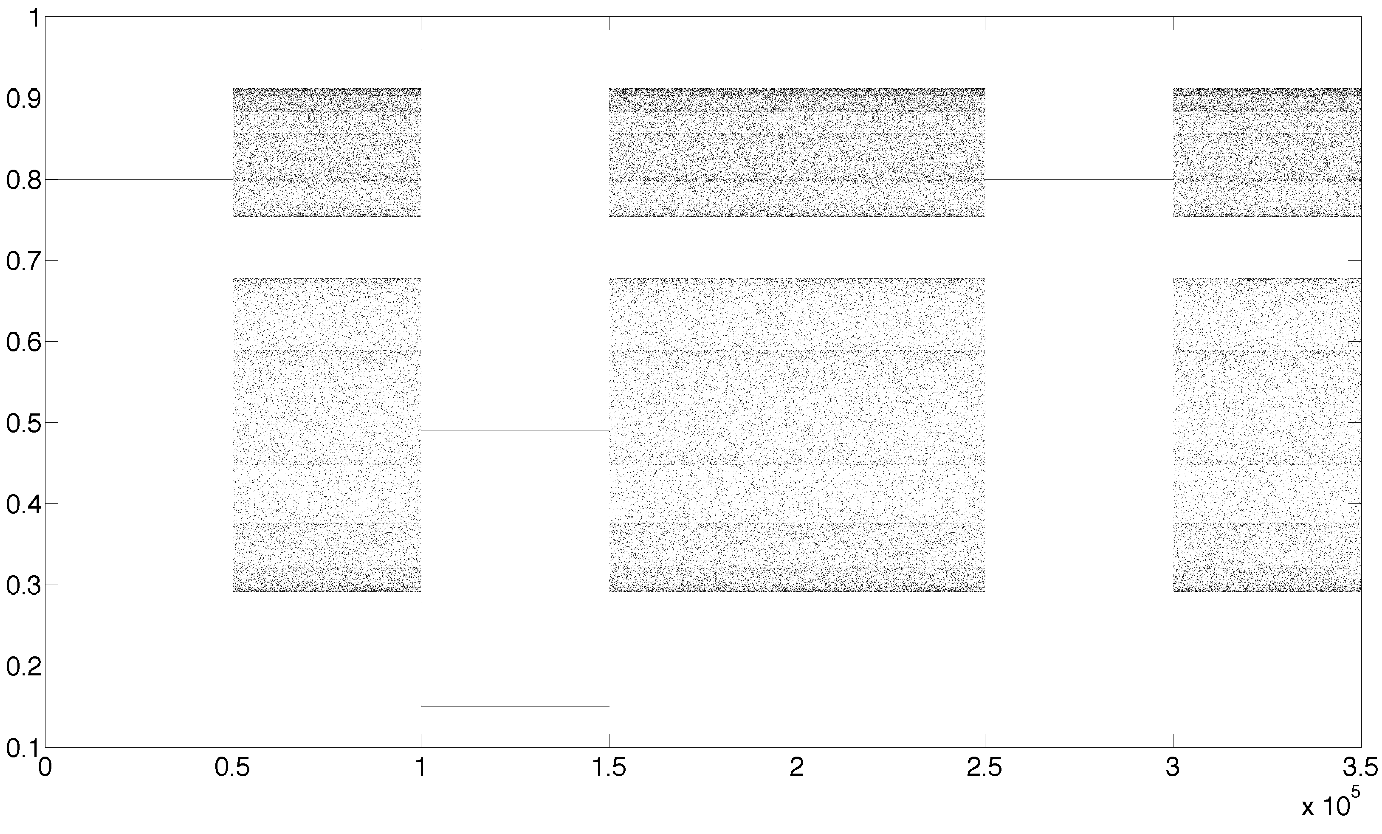
\includegraphics[width=\columnwidth]{unused-figs/ts-banded-alone}}
%%    {(a)}
%%
%%  \subfigure{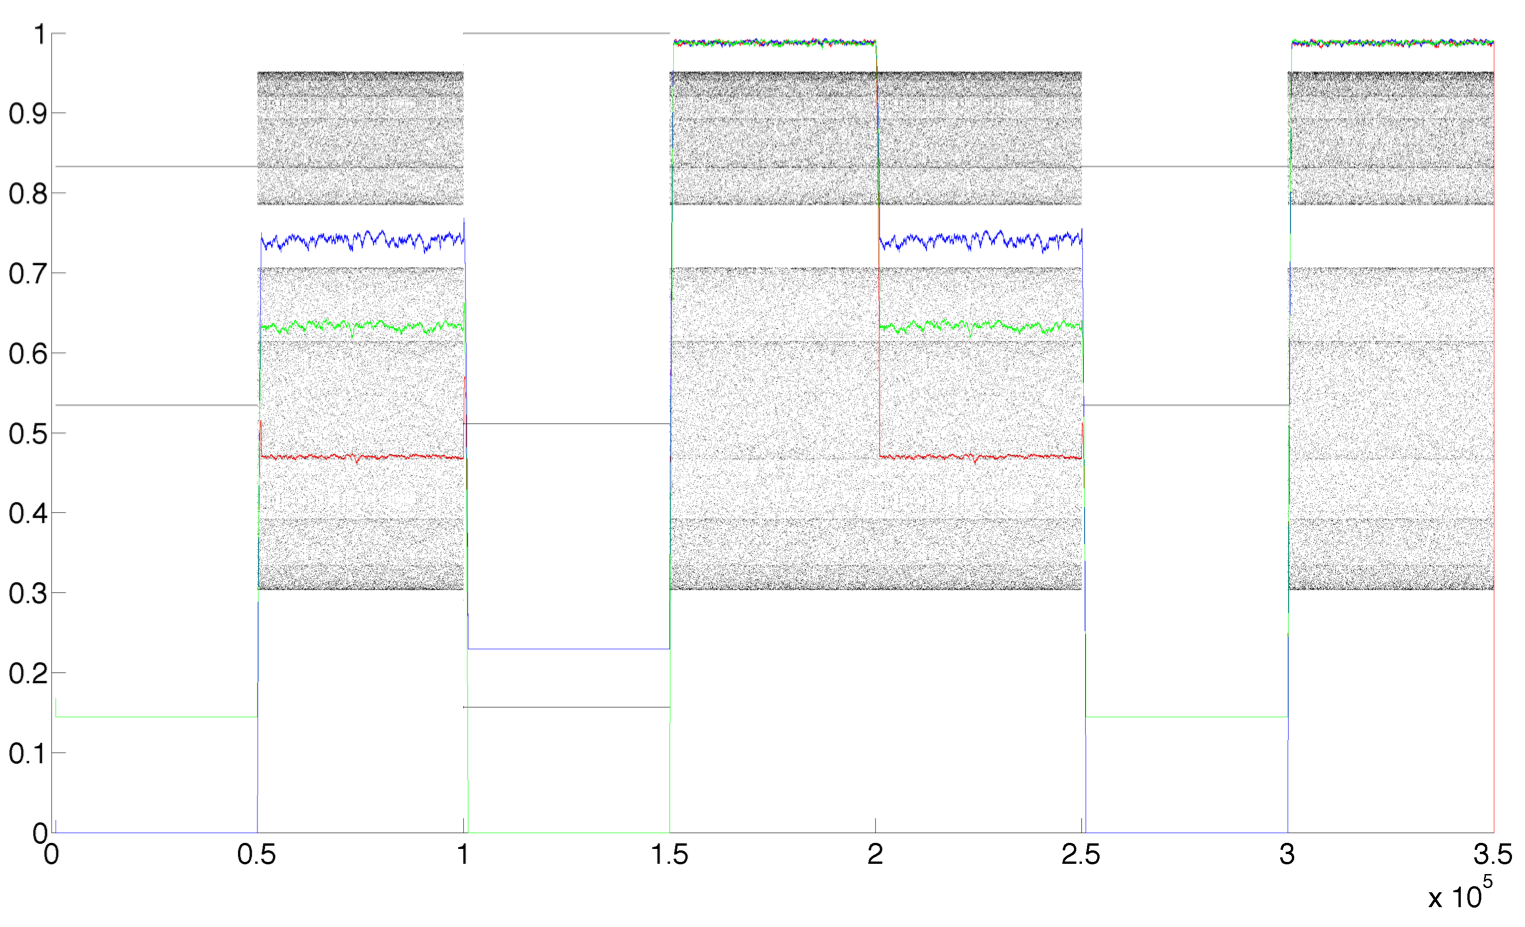
\includegraphics[width=\columnwidth]{unused-figs/ts-banded-pe}}
%%  {(b)}
%%  \caption{ (a) The concatenated time series discussed in Section~\ref{sec:concatenate}. (b) Plot of the concatenated time series from Section~\ref{sec:concatenate}, as well as permutation entropy as a function of time(blue,green and red curves). Each permutation entropy curve shown is calculated using $m=5$, however, the red,blue and green curve use a $\tau = 1,2,3$ respectively.}\label{fig:ts-banded}
%%\end{figure}
%
%
%
%
%
%
%and what is it good for with forward pointer to the other sections
%
%
%
%\subsubsection{Example: The transient Logistic map}
%In Section~\ref{sec:concatenate} we discussed a time series which stayed in a parameter regime for long amounts of time and then abruptly changed. As we showed, permutation was a great proxy to detect this change. Another type of parameter change that may occur in a physical system is constant parameter drift, i.e., some parameter slowly changes over time. To explore this type of parameter drift we construct the same time series as was used in \cite{cao2004det}. Iterate the logistic map, starting with $R=2.8$, then at every iteration increase $R$ by $10^{-5}$ until $R=4$. The time series, which can be seen in Figure~\ref{fig:translogistic} appears very similar to the standard bifurcation diagram for the Logistic map. The curves in red and blue are the permutation entropy calculated with $m=5$ and $\tau = 1,2$ (respectively).
%
% As we can see, as bifurcations occur in the dynamics the permutation entropy changes as well. An interesting feature of block calculations are the spikes that occur at bifurcation points. As the block begins to encompass multiple regimes, e.g., fixed point and  period two, permutations are being realized for both regimes. This overlap causes an increase in the time series complexity, and thus a spike in the permutation entropy. The dips you see in the second half correspond to bands of periodicity which occur between the chaos. It is worth noting, that the blue curve (permutation entropy with lag 2) does not go to zero in the period 2 parameter range. This is because this is not a true period 2 orbit but transient that is moving across \emph{several} period 2 orbits, thus it maintains a higher level of complexity, albeit still very low.
%
% This illustrates that permutation entropy can not only distinguish between instant (and drastic) parameter shifts but also very slow and gradual parameter drift.
%
%\begin{figure}[ht]
%  \centering
%  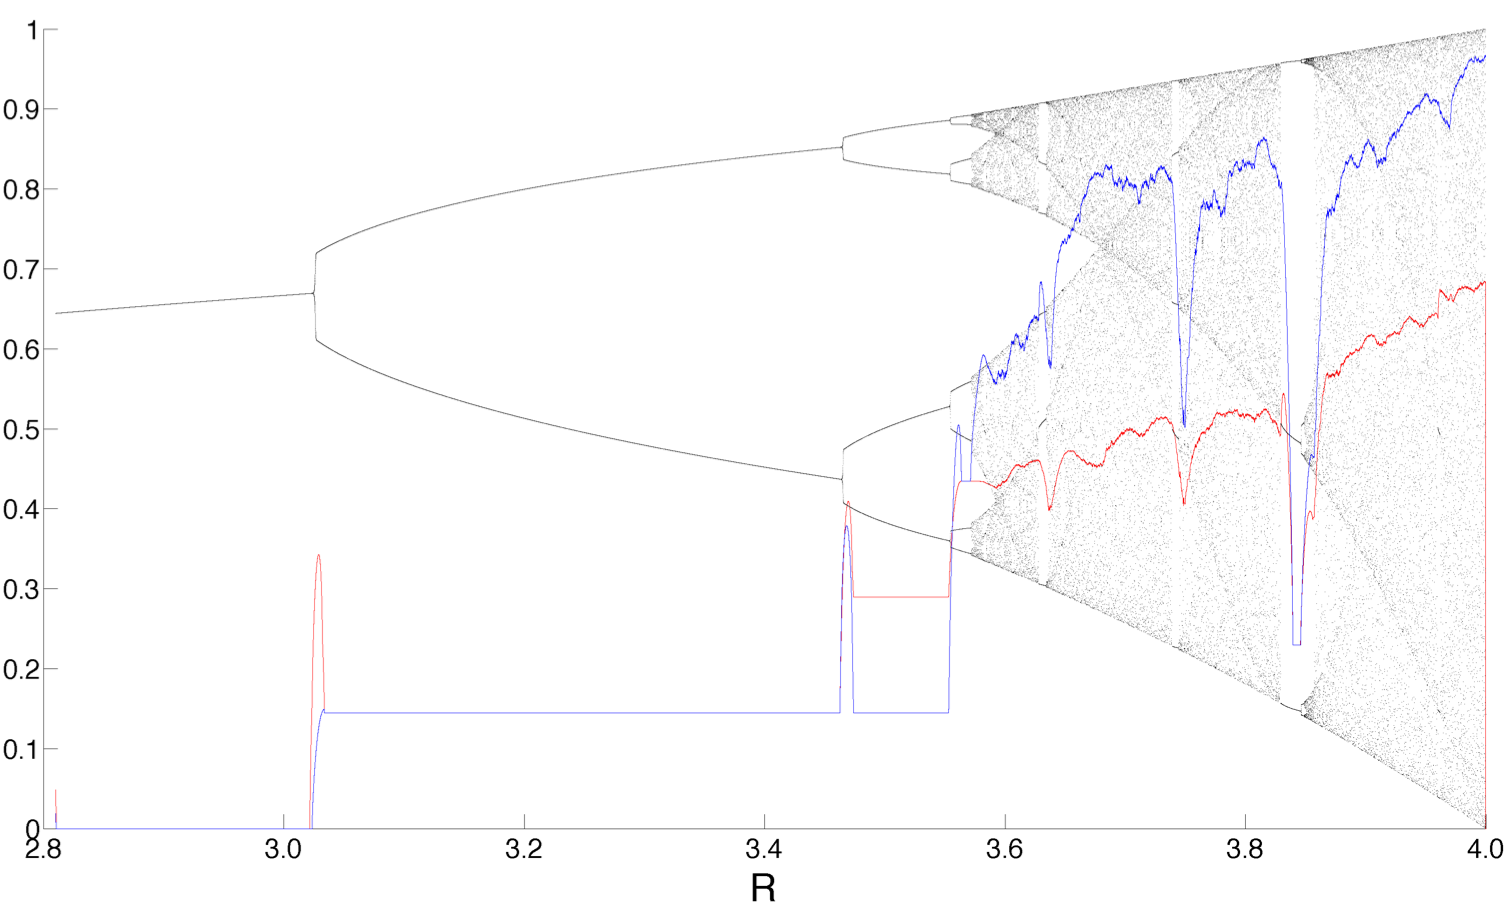
\includegraphics[width=\columnwidth]{unused-figs/tstranslog-perm}
%  \caption{Transient Logistic map time series and permutation entropy curves. Both permutation entropy curves are calculated with $m=5$, the red and blue correspond to $\tau = 1,2$ respectively.}
%  \label{fig:translogistic}
%\end{figure}
%%\begin{enumerate}
%%\item do with henon bifurcation. what happens near the broken chaotic window
%
%%\end{enumerate}
%
%
%The weighted permutation entropy for the \svd program is given in
%Fig.~\ref{fig:wwpe}. To generate this image a window of 5,000 values slid over
%the time series. Within each of those windows, the statistics over words of
%length 4 are computed and the WPE is calculated. The gray bands denote regions
%where the 5,000 value window overlapped visually-distinct regimes. It can be
%seen that the behaviors of the weighted permutation entropy vary between
%regimes. [[I think here it would be good to add a paragraph explaining the windowed WPE was used for regime choices on SVD...emphasizing  that over a time series permutation entropy fluctuates illustrating within a single time series different levels of complexity and predictability exist. Maybe point at some of the predicting predictability papers.]]
%
%%\begin{figure}[htbp]
%%  \centering
%%  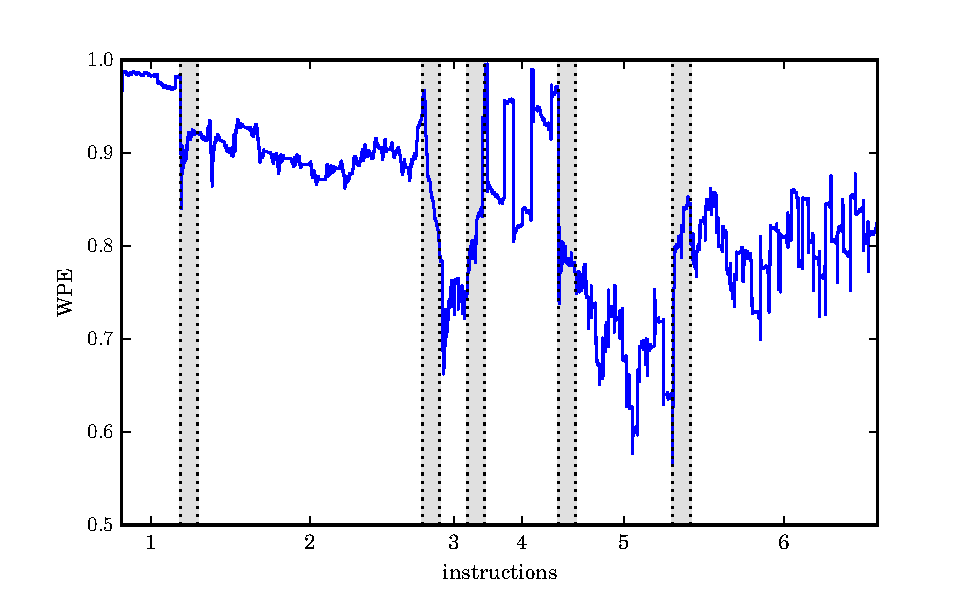
\includegraphics[width=1.0\textwidth]{figs/SVD_wwpe}
%%  \caption{[[Joshua: I think adding the colored SVD trace to this would be %good or putting it above this figure]]The weighted permutation entropy of %one run of SVD. The gray bands
%%    are regions where the window overlaps regimes. The window size used is
%%    $5,000 \times 100,000$ instructions and the word length is $4$.}
%%  \label{fig:wwpe}
%%\end{figure}
%
%
%%%FIGURE INTENT
%%This figure shows that entropy changs over time with the signal as well as why the regimes for \svd were chosen. 
%%%%%%%%%%%%%%%%%%
%\begin{figure}[htbp]
%  \centering
%  %\begin{subfigure}{0.3\textwidth}
%  %  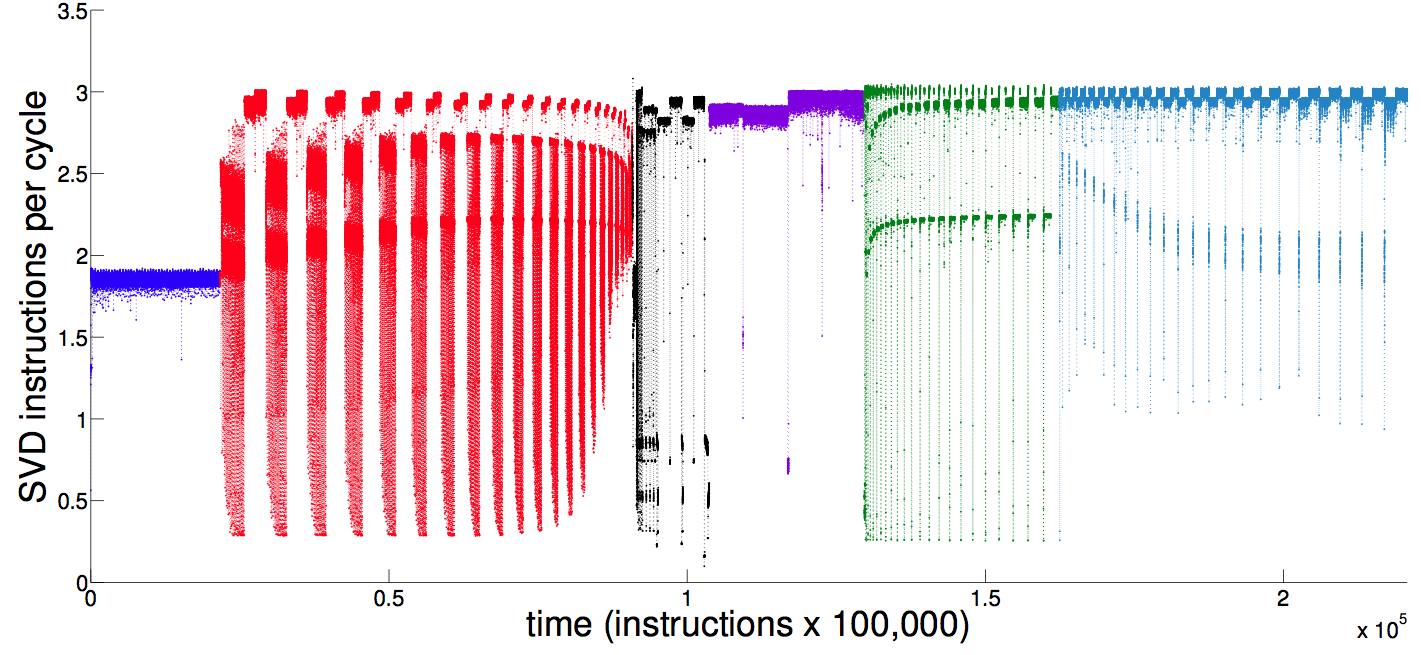
\includegraphics[width=0.3\textwidth]{figs/svdipcregimescolored.png}
%  %  \caption{The instructions per cycle of \svd. Each color corresonds to the different regimes as selected by rapid shifts in WPE, as seen in Figure \ref{fig:svd_wwpe}. From left to right each change in color represents a change in regime for 6 regimes in total. }
% %   \label{fig:svd_ts}
% % \end{subfigure}%
%  %\\
% % \begin{subfigure}{\textwidth}
%
% {\color{red}TODO: Put this image back in.}
%%Liz commented this image out temporarily so that her mac doesn't hang
%%when she scrolls past p12
%% We decided to skip the figure completely, since we took out
%% all stuff about PE as regime-shift detection.  
%% [[should add that as future work, though.]]
%  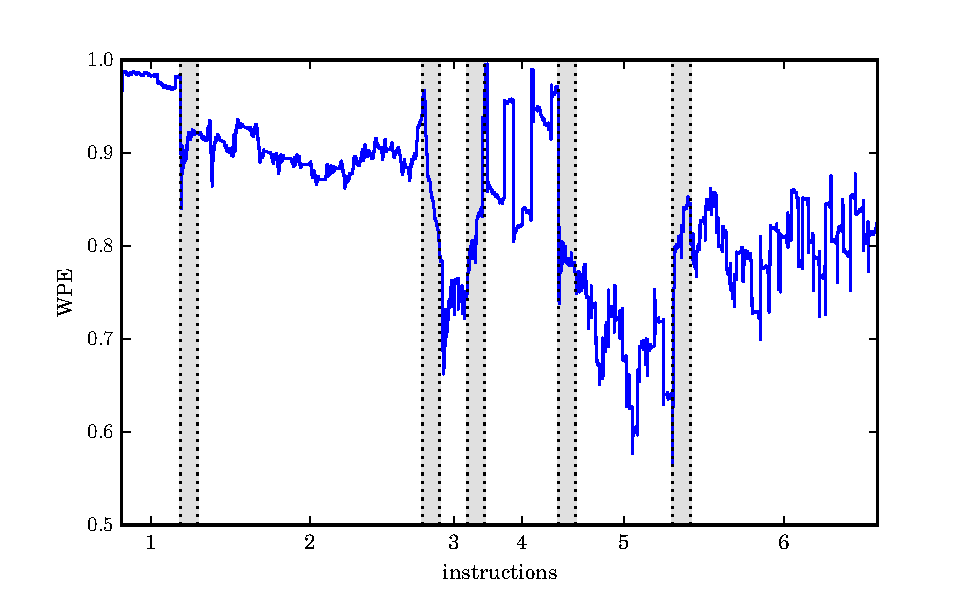
\includegraphics[width=\columnwidth]{figs/SVD_wwpe}
%  \caption{The weighted permutation entropy of one run of SVD. The gray bands are regions where the window overlaps regimes. The window size used is 5,000 $\times$ 100,000 instructions and the word length is $6$. For reference the instructions per cycle of \svd are plotted as a ghost behind this plot. Each color on the ghosted time series corresonds to the different regimes as determined by visual inspection. From left to right each change in color represents a change in regime for 6 regimes in total.}\label{fig:wwpe}
%\end{figure}
%



